\chapter{Introduction}
\label{cha:Introduction}

\TODO{"vom Allgemeinen zum Speziellen"}

\section{Motivation}
The RECENDT GmbH researches, develops and produces, among other technology areas, measurement systems employing optical coherence tomography. A key element of such OCT-systems are galvanometer-scanners.  These allow for analyzation of areas, instead of only point-wise measurements, by manipulating a laser-beam. This manipulation again, has to be controlled via two separate steering-voltages, one for manipulation in x- and y-axis. An existing mikrocontroller-board, providing sufficient precise and fast DACs, is to be programmed, to form the 'OCTane', a signal-generator for mentioned steering-voltages, controllable via USB. The resulting Firmware shall also incorporate a HAL, utilizing several other functionalities, the microcontroller has to offer. Optionally, adapted curves for the steering voltages shall be investigated to allow linear control over galvanometer-scanners in higher frequency ranges.

\section{Optical coherence tomography}
Optical coherence tomography (OCT) is an imaging measurement method for the analyzation of transparent and semi-opaque materials and shows similarities to the measurement processes via ultrasound or radar. The sample to be measured is subjected to an electromagnetic wave, the resulting 'echoes' are analysed with regard to their times of flight. From these run-times again,  the geometric structure is determined, including the layer structure of the sample and also the maximum penetration depth of the applied wave. This creates measured point with an in-depth resolution. Usually this EM wave is of a coherent broadband light source in the visible  up to the near infrared spectrum. Coherent means, that several wave-bundles of a light source must have a fixed phase relationship to eachother. This is necessary to obtain stable interference patterns.  For the Detection of the echoes, however, conventional opto-detectors or cameras do not suffice, on the one hand due to the propagation speed of light, on the other hand due to the low reflected light intensities. Therefore Interferometry is used to determine the depth of penetration of a photon, being reflected from the sample. In interferometry, a laser beam is split into two waves of half the initial optical power. One wave is sent on an optical reference path of known length, the other to the surface of the sample. The reflections, the returning waves are superimposed and, depending on the nature of the sample material, result in constructive or destructive Interference. This interference can be detected using an opto-detector[1], or a spectrometer[2] and used for further processing. A single measured point and its depth information about the material under test is called an A-scan. Aggregates a lot of A-scans along a line (X-direction) across the sample material, forms a B-scan and the aggregation of B-scans along a line in the Y direction a volume scan, i.e. a spatial, three-dimensional image of the sample material. Relevant parameters of OCT systems are the penetration depth, the axial and lateral measurement range, axial and lateral resolution and the measurement speed. While the penetration depth of ultrasound typically reaches a few centimeters and a resolution in the millimeter range, OCT allows only to look a few millimeters below the surface, but with micron resolutions. Measurable areas, or field-of-view, in ultrasound is in the order of centimeters, with OCT in the order of millimeters[1]. achievable speed al results from A-scan rates up to 100kHz. The term 'optical coherence tomography' results on the one hand from the coherent light source. The other two parts of the name, 'tomos' means slice or section, and 'graphein' stand for writing or drawing, and both come from Greek. They reflect that the resulting image is assembled from individual slices or sectional images. 
The manipulation of the light beam along the mentioned lines takes place with rotatably mounted mirrors, one for the X one for the Y direction. The faster this rotation is possible, the faster OCT-images can be created. One widespread technical realization, allowing very fast rotation of the mirrors called a galvanometer-mirror or -scanner.

\section{Galvanometer-Scanners}
% \TODO{Buedln ausm WIA-Papaer holen} \\
\TODO{'scanner' statt 'mirror'} \\
Galvanometer scanners (colloquial: galvos) are highly dynamic opto-mechanical components, based on the classic galvanometer according to Hans Christian Oersted: A rotatable, magnetizable object, e.g. a magnetic needle, that will be deflected from its position in the proximity of a current-carrying conductor. The low sensitivity of the effect on the current is improved by a high number of windings of the electric conductor around the deflectable object, creating an electrical Inductance, a coil. The non-linear connection between current and deflection angle can be linearized to a first-order approximation, by placing the coil between a rigidly potitioned iron-cylinder inside and a permanent-magnet, which is arranged outside the coil[2]. 
If this classic Galvanometer is equipped with a mirror as a rotatable object, optical paths, specifically: the beam-path of a point light source, can be manipulated in one space dimension. Feaseable for technical applications is, that this manipulation can be controlled reasonably linear by the current or voltage at the galvo coil. With the galvanometer-scanner employed for this master-thesis, power-electronics for the conversion of control signals to the required coil-currents and -voltages were already included. Therefore, furthermore, only 'control signals' will be discussed, instead of currents and voltages. A combination of two galvanometer scanners in a suitable geometric arrangement, irradiated with a point laser, allows to manipulate this point in two dimensions. Such an arrangement is shown in fig. []. At sufficient speed with which the laser point is deflected, 2-dimensional contours can be projected, resulting in a 'stationary' image for the human eye. It shall be noted, that only closed geometric figures are possible, as long as the light source itself cannot be turned off. These components are commercially available as laser scanner and used for light effects at music events, art installations and in discotheques. Applied to OCT-systems, on the other hand, galvanometer scanners are used to expand measurement from a single point of interest. Deflecting mentioned coherent light source of an area of an examined sample, allows for two-dimensional analysis of the sample. If a dedicated x- and a y-galvo are to be steered with a slow and a fast ramp, respectively, this results in a rectangle on the sample, which is the desired 'image shape' of the laser dot for OCT systems. In this way, samples can be scanned in a grid pattern.

\begin{figure}[h!]	\centering	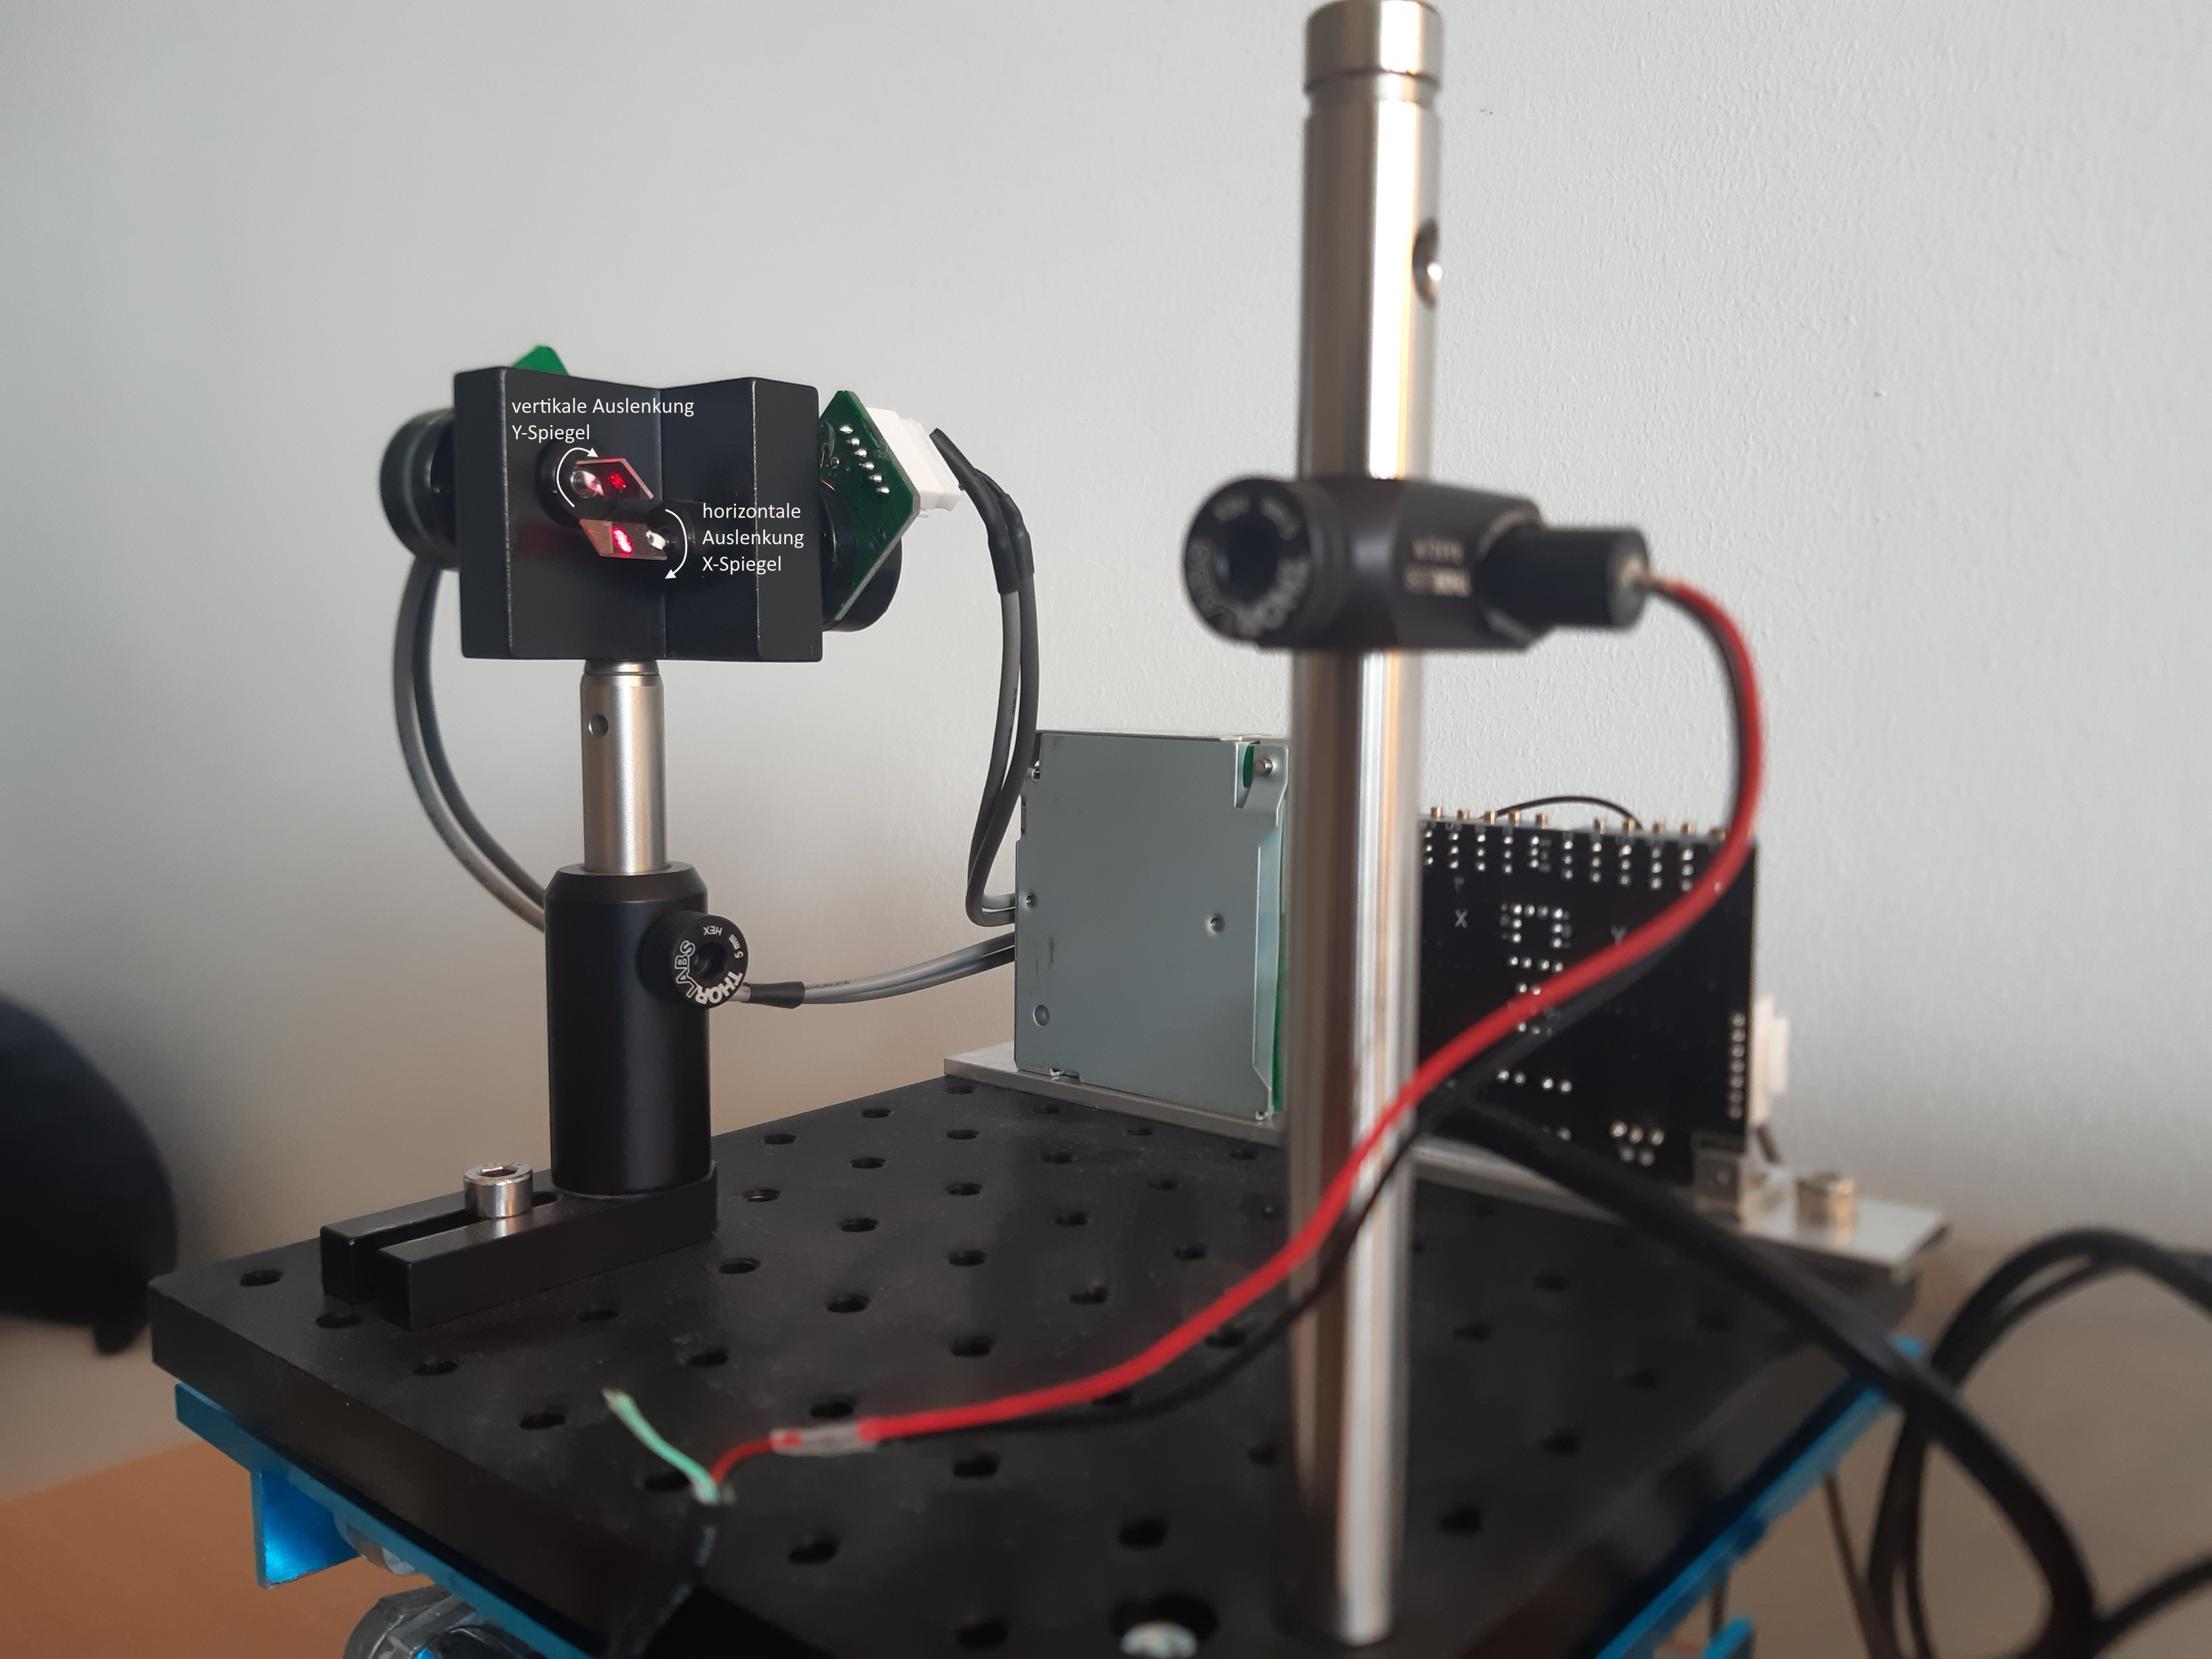
\includegraphics[width=\textwidth]{images/DetailGalvoOn.jpg}	\caption{DetailGalvoOn}	\label{DetailGalvoOn}	\end{figure}
\begin{figure}[h!]	\centering	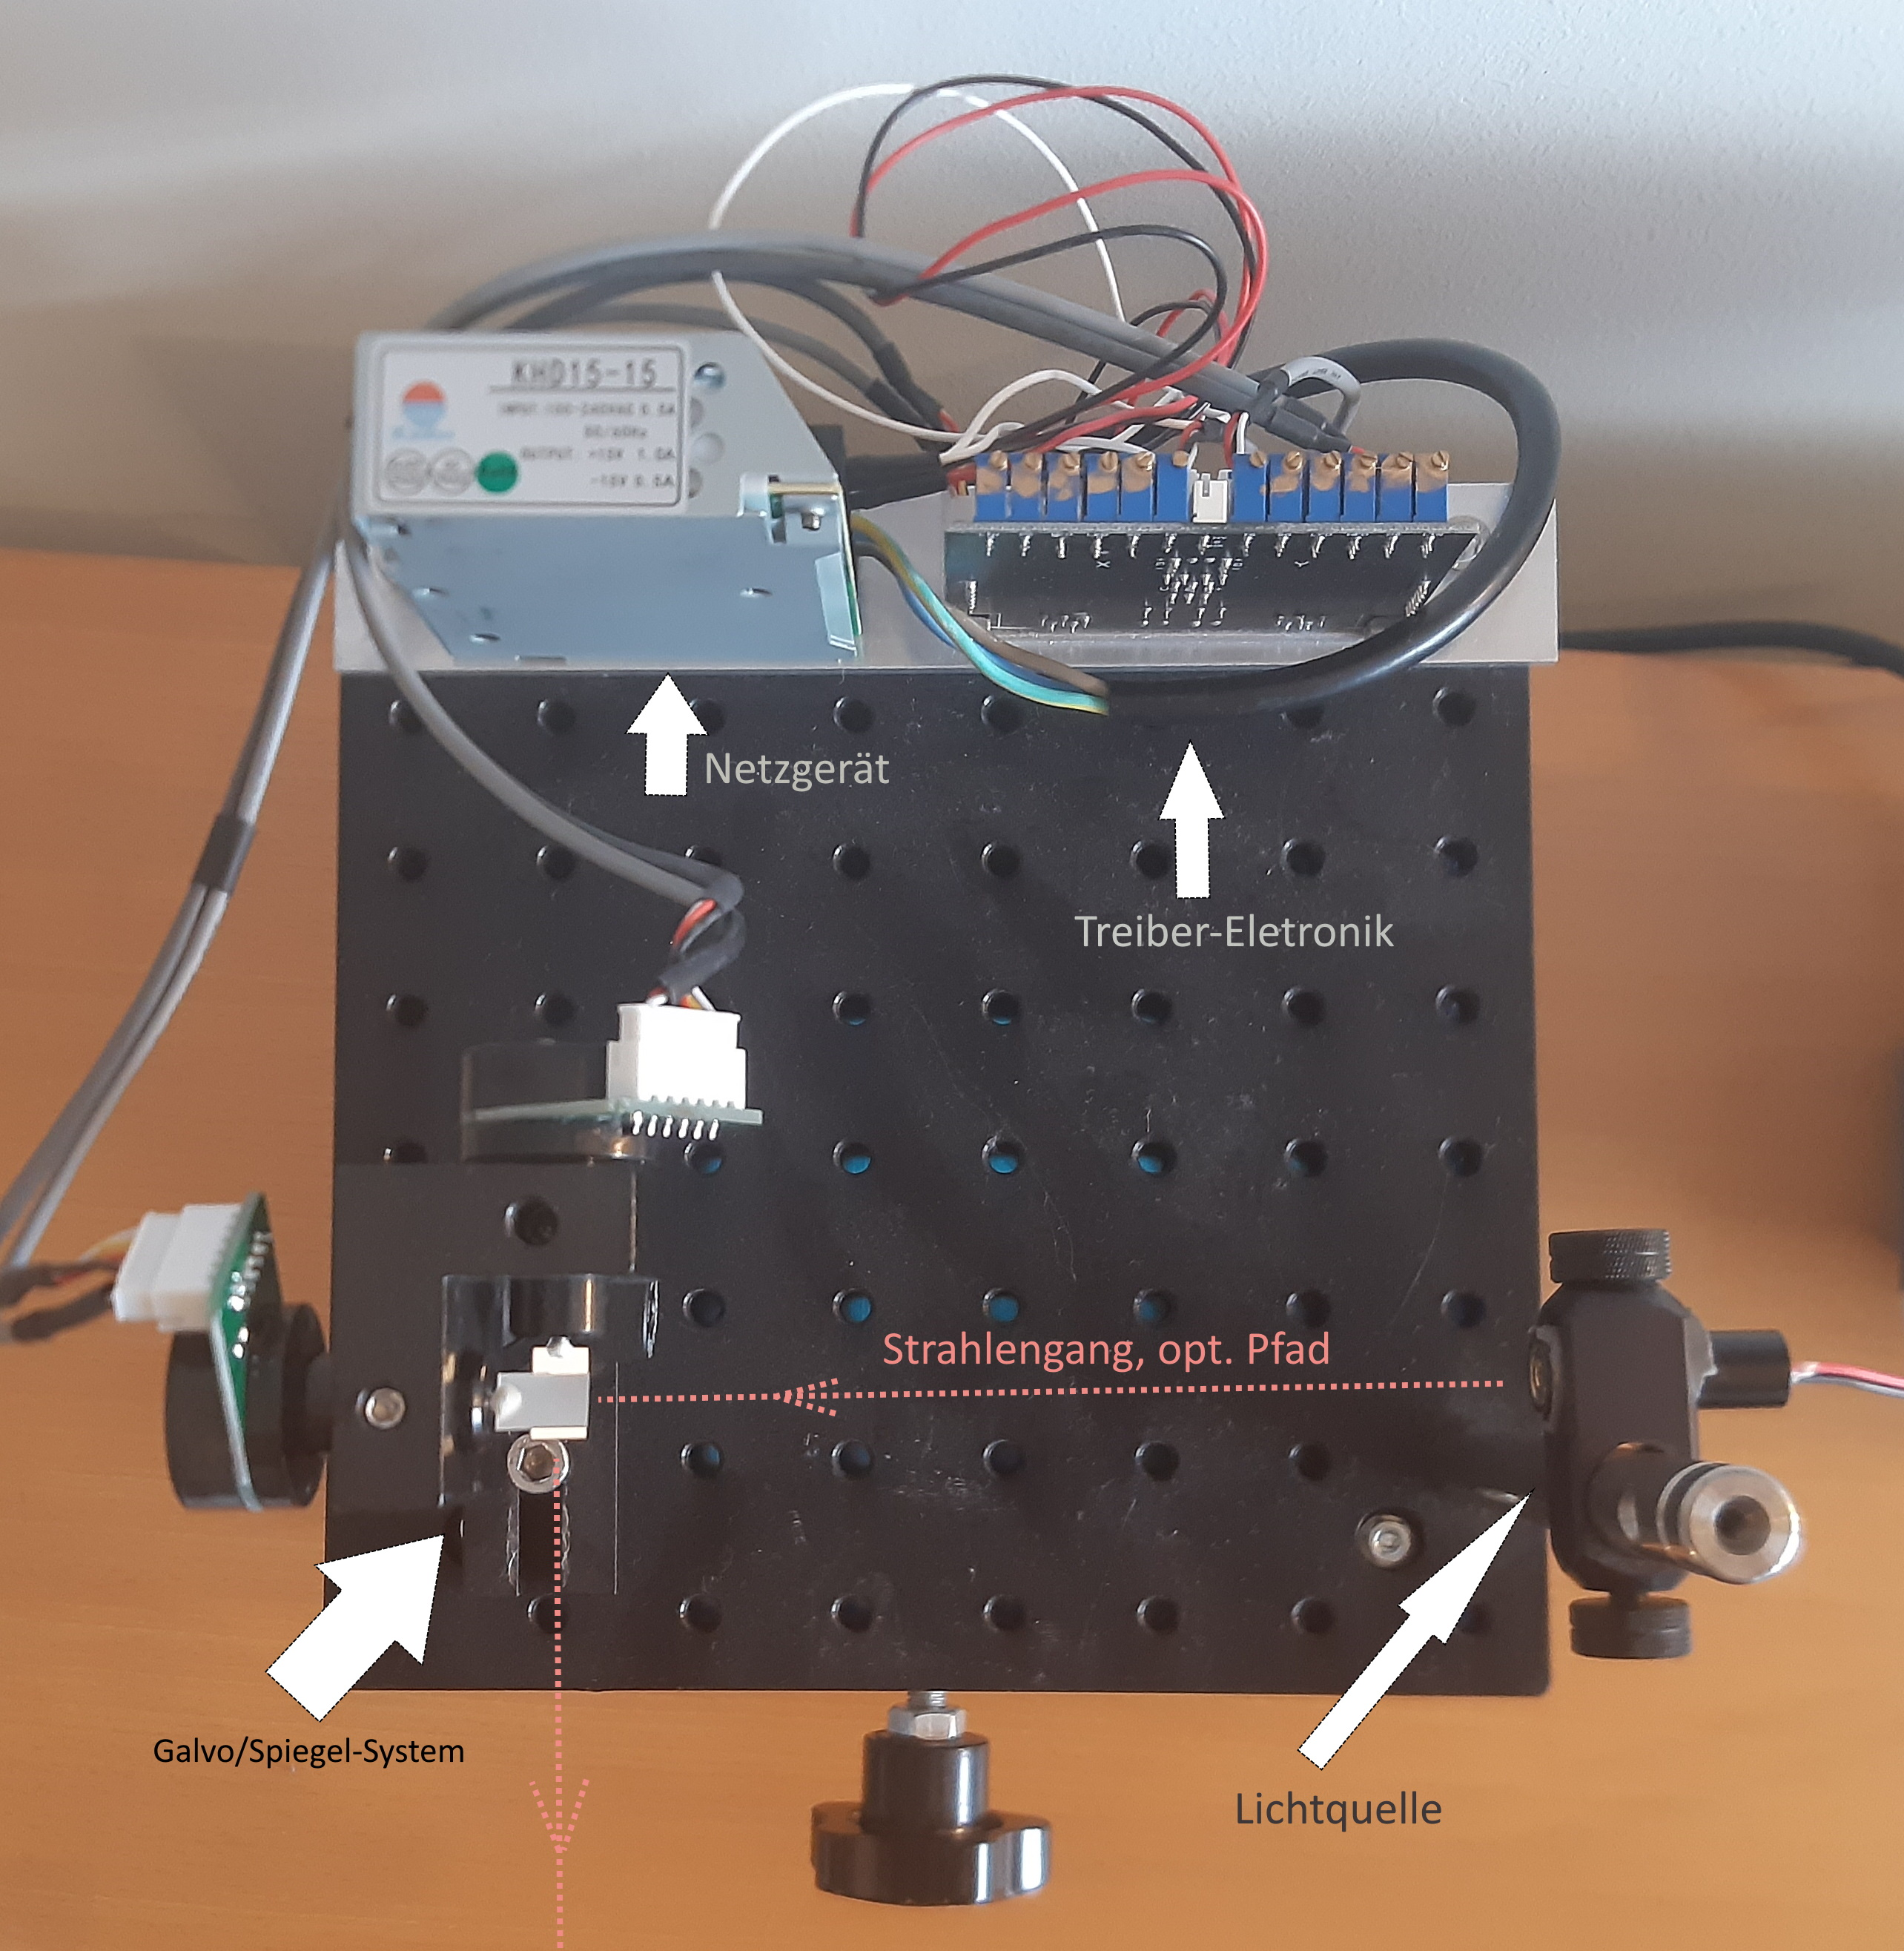
\includegraphics[width=\textwidth]{images/DutTop02.jpg}	\caption{DutTop02}	\label{DutTop02}	\end{figure}

\section{Control of Galvanometer-Scanners}
Commercially available Galvanometer-Scanners usually allow control in the form of analog voltage inputs with a range of $\pm$ 10Volts. The angle of the rotated mirror follows that control-voltage in a linear manner for sufficiently low frequencies. The signal-forms to result in the rectangular scan-grids, as described in the previous section, are depicted in Fig.~\ref{GalvoRamps01}. To achieve these signals, a mikrocontroller-board was designed, including 16-bit-DACs, USB-PHY and coaxial Trigger-IOs, among other features. To utilise these features and form an arbitrary signal generator for mentioned ramp-signals, a firmware is necessary. This should be done in a fashion employing quality-assurance during the implementation-process, as well as the verification-phase of the firmware and its supporting hardware. Aside from signal-generation and USB-connectivity, additional features are desirable, such as user-controllable Relays, utilisation of watchdog-timer, UART-, I2C- and SPI-ports as well as analog inputs. The combination of hard- and firmware will be called OCTane.
\begin{figure}[h!]	\centering	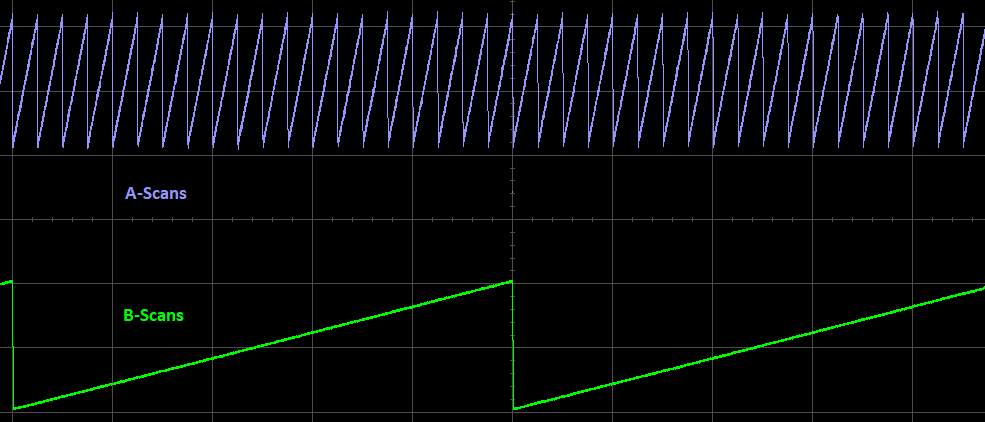
\includegraphics[width=\textwidth]{images/GalvoRamps01.png}	\caption{GalvoRamps01}	\label{GalvoRamps01}	\end{figure}
\TODO{block-schematic: PC -> OCTane -> 2xDAC -> Galvo-Driver} \\
This leads to the scientific problem at hand: 
\begin{center} {\bf How can measures of quality be applied to a bare-metal firmware?}
\end{center}
\subsection{optional: adapted steering curves}
...fliegt wohl raus
\TODO{Modell ausm Paper per flachheitsbasierter Reglung auf Steuer-rampen draufrechnen}
% \textcolor{gray}{  }
